
\documentclass[11pt]{article}
\usepackage[paper=letterpaper, margin=.5in]{geometry}
\linespread{1.5}
\pdfpagewidth 8.5in
\pdfpageheight 11in

%%% Packages
% First four - AMS (american mathematical society). General math goodness. I use the align* enviorment in particular
% multirow, multicol allow for certain kinds of tables
% enumerate lets you determine the style of the counter for the enumerate enviorment
% graphicx lets you include pictures
% listings lets you stick in blocks of code
% placeins defines "\FloatBarrier", which stops tables from moving around
\usepackage{amsmath, amscd, amssymb, amsthm, multirow, multicol, enumerate, graphicx, listings, placeins, caption} 
\captionsetup{font={small,singlespacing},margin=1cm}
\newcommand{\Z}{\mathbb{Z}}
\newcommand{\R}{\mathbb{R}}
\newcommand{\Q}{\mathbb{Q}}
\newcommand{\C}{\mathbb{C}}
\newcommand{\N}{\mathbb{N}}
\newcommand{\V}{\mathbb{V}}
\newcommand{\U}{\mathcal{U}}
\newcommand{\del}{\partial}
\newcommand{\real}{\textrm{Re }}
\newcommand{\imag}{\textrm{Im }}
\newcommand{\pd}[2]{\frac{\partial #1}{\partial #2}}
\newcommand{\deriv}[2]{\frac{d #1}{d #2}}
\newcommand{\sumk}{\sum_{k=1}^\infty}
\newcommand{\sumj}{\sum_{j=1}^\infty}
\newcommand{\sumn}{\sum_{n=0}^\infty}
\newcommand{\summ}[2]{\sum_{k=#1}^{#2}}
\newcommand{\sig}[1]{\sum_{#1 =1}^\infty}
\newcommand{\un}[1]{\bigcup_{#1 =1}^\infty}
\newcommand{\inter}[1]{\bigcap_{#1 =1}^\infty}
\newcommand{\ip}[2]{\langle #1, #2 \rangle}
\newcommand{\ipxu}{\langle x,u_j \rangle}
\newcommand{\uj}{\{u_j\}_{j=1}^\infty}
\newcommand{\B}{\mathcal{B}}

\newcommand{\p}{\mathrm{P}}
\newcommand{\E}{\mathrm{E}}
\newcommand{\var}{\mathrm{Var}}
\newcommand{\cov}{\mathrm{Cov}}
\newcommand{\diag}[1]{\mathrm{diag}\{#1\}}
\newcommand{\ST}{mbox{ s.t. }}

\newcommand{\x}{\bf x}

\newcommand{\Example}{\noindent {\bf Example. \quad} }
\newcommand{\Proof}{\noindent {\bf Proof: \quad} }
\newcommand{\Remark}{\noindent {\bf Remark. \quad} }
\newcommand{\Remarks}{\noindent {\bf Remarks. \quad} }
\newcommand{\Case}{\noindent {\underline{Case} \quad} }

\newcommand{\st}{ \; \big | \:}

\newcommand{\deuc}{d_{\mathrm euc}}
\newcommand{\dtaxi}{d_{\mathrm taxi}}
\newcommand{\ddisc}{d_{\mathrm disc}}
\newtheorem{theorem}{Theorem}[section]
\newtheorem{lemma}[theorem]{Lemma}
\newtheorem{proposition}[theorem]{Proposition}
\newtheorem{corollary}[theorem]{Corollary}
\theoremstyle{definition}
\newtheorem{definition}[theorem]{Definition}
\newtheorem{example}[theorem]{Example}
\DeclareMathOperator*{\argmin}{arg\min}

\newcommand{\hwhead}[1]{#1 \hfill Aaron Maurer \vspace{2mm} \hrule \vspace{2mm}}

\begin{document}
\title{Using Probabilistic Knockoffs of Binary Variables to Control the False Discovery Rate}
\author{Aaron Maurer}
\maketitle
%%%%%%%%%%%%%%%%%%%%%%%%%%%%%%%%%%%%%%%%%%%%%%%%%%%%%%%%%%%%%%%%%%%%%%%%%%%%%%%%%%%%%%%%%%%%%%%%%%%%%%%%%%%%%%%%%%%%%%%%%%%%%%%%%%%%%
\section{Introduction}
    Variable selection is an essential problem to fitting a regression model. For linear regression, the knockoff filter (Barber and Cand\`{e}s, 2014) offers a method of exact FDR control. However, the method as originally formulated does not extend to other generalized linear models such as logistic regression. This paper offers an extension of this method which will work with binary features in the context of linear regression, but also will extend to other GLMs.  
    
\subsection{Knockoff Filter}
    Let us consider the consider the usual setting for linear regression, where $n$ observations of a variable of interest $y$ arise from the model
    \[\mathbf{y} = X\beta + \mathbf{z}\]
    where $\mathbf{y}\in\R^n$ are the observed values of $y$, $X \in \R^{n\times p}$ is the matrix of predictor variables, $\beta\in\R^p$ are the unknown coefficients, and $\mathbf z$ is Gaussian noise. It is important to note that a intercept vector $\mathbf 1$ is not included in $X$. For the purpose of this paper, only the case where $2p\leq n$ will be considered, though the methods can be extended to $p\leq n$. I will to refer the $j$th column of $X$ as $X_j$, which is $n$ observations of the random variable $x_j$. The random variable $x_j$ is in turn $j$th entry of the random vector valued variable $\mathbf x$. In the situation where $\beta$ is sparse and there is reason to expect that $x_j$ and $y$ are uncorrelated for many $j$, the knockoff filter is a method to select a subset of the $x_j$ which are likely correlated with $y$. \par
    The method specifically seeks to control the false discovery rate (FDR), which is the expected portion of some selection of $x_j$ which are, in fact, uncorrelated with $y$. For a procedure which chooses a subset of variables $\hat S\subseteq \{1,\ldots,p\}$, this is defined as  
    \[ \textrm{FDR} = \E\left[\frac{\vert{\{j: \beta_j=0 \; \& \; j\in\hat S\}}\vert}{\max\{\vert{\hat S}\vert,1\}} \right] \]
    FDR is controlled at level $q$ if FDR is less than $q$ irrespective of the coefficients $\beta$. \par

    The knockoff filter achieves FDR control in several steps, the first of which is creating a set of `knockoff' features $\tilde X_j$ which imitate the original $X_j$ while being less correlated with $y$. In particular, the matrix of knockoffs $\tilde X$ has the same internal correlation structure as $X$, the knockoff feature $\tilde X_j$ has the same correlation with other $X_i$ as $X_j$ does, but the correlation between $\tilde X_j$ and $X_j$ is minimized. In other words, where $ G := X^TX$, 
    \[ \tilde X^T\tilde X=G \textrm{ and } \tilde X^T X = G - \diag{\mathbf s}\]
    for some vector $s\in \R^p$ such that, where $\diag{G}$ is the vector made from the main diagonal of $G$, $\diag{G} - \mathbf s$ is small. Since $\tilde X_j$ and $X_j$ have relatively low correlation, as long as $X_j$ is created independently of $\mathbf y$, $\tilde X_j$ will have lower correlation with $\mathbf y$ than $X_j$. In the case where $X_j$ is uncorrelated with $\mathbf y$, $\tilde X_j$ will also be uncorrelated with $\mathbf y$. How these knockoffs are actually generated will be described shortly.\par
    The second step is to fit a series of Lasso model of $\mathbf y$ on the combined design matrix $X_L=[X \; \tilde X]$ so as to determine the largest value $\lambda$ at which the coefficient for each $X_j$ and $\tilde X_j$ is nonzero. The subscript $L$ refers to the large design matrix with both features and knockoffs. \footnote{Other statistics besides the $\lambda$s can also be used in the knockoff method, but are not considered in this paper} Recall, for a given $\lambda$, the estimated coefficient from the Lasso regression will be 
    \[ \beta(\lambda) = \argmin_\mathbf b \left\{\frac{1}{2}\|\mathbf y - X_L\mathbf b\|^2_2 + \lambda\|b\|_1 \right\}\]
    In the general case, the coefficient for one feature in a Lasso regression being first nonzero for a larger value of $\lambda$ than another feature is an indication that the first feature is a stronger predictor of the outcome than the second. Thus, since, by construction, the knockoff features are weaker predictors than the originals, we would expect the original features to have nonzero coefficients sooner than the knockoff features when the original is a valid predictor. On the other hand, since $\beta(\lambda)$ only depends on $X_L$ through the sufficient statistics $G_L=X_L^TX_L$ and $X_L^T\mathbf y$, for null predictors, the coefficients of the original features won't enter any sooner on average than knockoff feature. This can be seen by switching a null $X_j$ with $\tilde X_j$; by construction, $G_L$ will be unaltered, while $\E\left[X_L^T\mathbf y\right]$ will also be unchanged, since $\E[X_j^T\mathbf y]=\E[\tilde X_j^T\mathbf y]=0$. \par
   This observation leads to the final step. Let $Z_j$ be the largest $\lambda$ such that feature $j$ has a nonzero coefficient and $\tilde Z_j$ the largest $\lambda$ such that knockoff $j$ has a nonzero coefficient. Then, define $W_j$ as 
   \[ W_j = \begin{cases}   Z_j         &\mbox{if } Z_j>\tilde Z_j \\ 
                            -\tilde Z_j &\mbox{if } Z_j<\tilde Z_j \\
                            0           &\mbox{if } Z_j=\tilde Z_j \\
            \end{cases} \]
            When $X_j$ is a null predictor, $W_j$ will be symmetrically distributed around zero, and when $X_j$ is true predictor, it will have a distribution skewed positive. Since $W_j$ with large positive values are more likely to be true predictors, the knockoff filter selects the variables $\{j:W_j\geq T\}$, where $T$ is a threshold defined as
            \[ T = \min\left\{ t>0 \;: \; \frac{\vert\{j:W_j\leq -t\}\vert}{\max\{\vert\{j:W_j\geq t\}\vert,1\}}\leq q \right\} \]
            Basic logic of this method is fairly simple. Let $N_h(t)$ be the random variable for the number of null predictors with $W_j\leq t$, $N_l(t)$ be the number of null predictors with $W_j\geq t$, and $V_l(t)$ \& $V_h(t)$ be the similar number of true predictors. Since the null $W_j$ are symmetrically distributed around $0$, $\E[N_l(t)]=\E[N_h(t)]$. Thus,
            \begin{align*}
                q &\geq \E\left[ \frac{\vert\{j:W_j\leq -t\}\vert}{\max\{\vert\{j:W_j\geq t\}\vert,1\}} \right] \\
                q &\geq \E\left[ \frac{N_l(t) + V_l(t)}{\max\{N_h(t) + V_h(t),1\}} \right] \\
                q &\geq \E\left[ \frac{N_l(t)}{\max\{N_h(t) + V_h(t),1\}} \right] \\
                q &\geq \E\left[ \frac{N_h(t)}{\max\{N_h(t) + V_h(t),1\}} \right] \\
                q &\geq \textrm{FDR}
            \end{align*}
            So FDR is controlled, and since $V_l(t)$ will tend to be small, it should be controlled fairly tightly.

\subsection{Original Knockoff Features}
    The original formulation of the method offers two similar methods of constructing knockoffs. Both of these will, by construction, have exactly the property that
    \[ \tilde X^T\tilde X=G \textrm{ and } \tilde X^T X = G - \diag{\mathbf s}.\]
    For both methods, the first step is to normalize the matrix $X$ such that $X_j^TX_j=1$ for all $j$. Then, let the Gram matrix of $X_L$ is
    \[ G_L= [X\; \tilde X]^T[X\; \tilde X] = \left[ \begin{array}{cc} G & G - \diag{\mathbf s} \\ G - \diag{\mathbf s} & G \end{array}\right] \]
    $A$, the Schur complement of $G$ in $G_L$ can be calculated as 
    \[ A = 2\,\diag{\mathbf s} - \diag{\mathbf s}G^{-1}\diag{\mathbf s} \]
    For $G_L$ to exist, $G_L$ must be positive semi-definite, which happens if and only if $A$ is positive semi-definite, which happens in turn if and only if\footnote{A fleshed out version of this argument can be found in the original knockoff paper} 
    \[ \diag{\mathbf s} \succeq 0  \; \textrm{ and } \; 2G - \diag{\mathbf s} \succeq 0 \]
    Given this is true, $A$ can be factored as $A=C^TC$. Combining this with a satisfactory $\mathbf s$ and an orthonormal matrix $\tilde U\in\R^{n\times p}$ such that $\tilde U^T X = 0$, a $\tilde X$ fulfilling the desired properties can be calculated as 
    \[ \tilde X = X(I-G^{-1}\,\diag{\mathbf s}) + \tilde UC\]
    As mentioned above, $\mathbf s$ should be chosen so as to make $\diag{G}-\mathbf s$ small. Since each $X_j$ has been normalized, this means that $\diag{G}=\mathbf 1$, so $\mathbf 1 - \mathbf s$ should be minimized in accordance with the restrictions on $\mathbf s$. The two methods differ in how $\mathbf s$ is chosen:
    \begin{itemize}
        \item \textit{Equi-correlated knockoffs}: Each original features is set to have the same correlation with its knockoff by setting $\mathbf s = 2\min\{\lambda_{min}(G),1\}\mathbf 1$. For all simulations in this paper, this was the method used.
        \item \textit{SDP knockoffs}: The $\mathbf s$ which minimizes the average correlation between knockoff and original features can be found via a semi-definite programing problem:
            \begin{center}
                \begin{tabular}{r l}
                    minimize & $\|\mathbf1-\mathbf s\|_1$ \\
                    subject to & $ 0 \preceq \diag{\mathbf s} \preceq 2G $
                \end{tabular} 
            \end{center}
            This method is significantly more computationally intensive. 
    \end{itemize}
     
\subsection{Binary Knockoffs}
    Though the ``original" knockoff method, described above, achieves the exact desired knockoff properties, the individual values in the vector $X_j$ will have little relation to the individual values in $X_j$. In particular, these values will often have very different empirical distributions. This effect is particularly noticeable when the random variable $x_j$ is discrete but $\tilde X_j$ does not even consist of the same set of values. The end result is that for variable selection for other generalized linear models, which do not have the same sufficient statistics as linear regression which knockoffs are designed to hit, the original knockoffs will fail to control FDR. \par
    Thus, this paper offers a new method of generating knockoffs which should offer superior performance with other GLMs. In this new method, the matrix of knockoff features $\tilde X$ will be generated by row from a random vector valued variable $\mathbf{\tilde x}$, each entry $\tilde x_j$ of which will have the property $\tilde x_j \sim x_j$. This random variable will also abide by a relaxation of the original knockoff condition:
    \[ \E[\mathbf{\tilde x}^T\mathbf{\tilde x}]=G \; \textrm{ and } \; \E[\mathbf{\tilde x}^T \mathbf x \st \mathbf x] = G - \diag{\mathbf s}\]
    This will ensure that, at the very least, these knockoffs are a suitable replacement for the original knockoffs for linear regression. \par
    Generating such knockoffs for a completely general case of any $\mathbf x$ is likely infeasible. However, in the specific case where $\mathbf x$ is a random binary vector variable, this paper will demonstrate a method to generate such knockoff variables. Since binary data is extremely common in many areas, this will hopefully serve as a useful tool.

\subsection{Paper Organization}
The rest of this paper will be organized in the following fashion:
\begin{itemize}
    \item Section 2 will go into more detail about how the original knockoffs breakdown with generalized linear models. In particular, several simulations will demonstrate how they breakdown.
    \item Section 3 will develop the method and theory for generating binary knockoffs.
    \item Section 4 will discuss tests of Binary knockoffs in simulation, both in comparison to the original knockoffs with Lasso and for logistic regression by itself.
    \item Section 5 is the final section, and will contain discussion of the results as well as areas for further work.
\end{itemize}

\section{Issues With Deterministic Knockoffs} 
    The knockoff filter and $W$ statistics have a very natural extension to generalized linear models. Here, where $l(\beta\st X, \tilde X)$ is the log likelihood of coefficients $\beta$ given the model, the $L1$ regularized regression model will have estimated coefficient vector
    \[ \beta(\lambda) = \argmin_\mathbf b \left\{l(\beta\st X, \tilde X) + \lambda\|b\|_1 \right\}\]
    The $Z_j$ and $\tilde Z_j$ are then, once again, the largest $\lambda$ such that the given original or knockoff feature has a positive coefficient, and then $W_j$ is constructed exactly as before. The problem with this is that if the given GLM doesn't have the same sufficient statistics as linear regression, there is no theoretical guarantee that the knockoff filter will control FDR. This is since, for null $X_j$, there is no theory to guarantee the $Z_j$ and $\tilde Z_j$ are exchangeable, and thus $W_j$ is not guaranteed to be symmetrically distributed around $0$. \par
    \begin{figure}[h]
        \begin{center}
        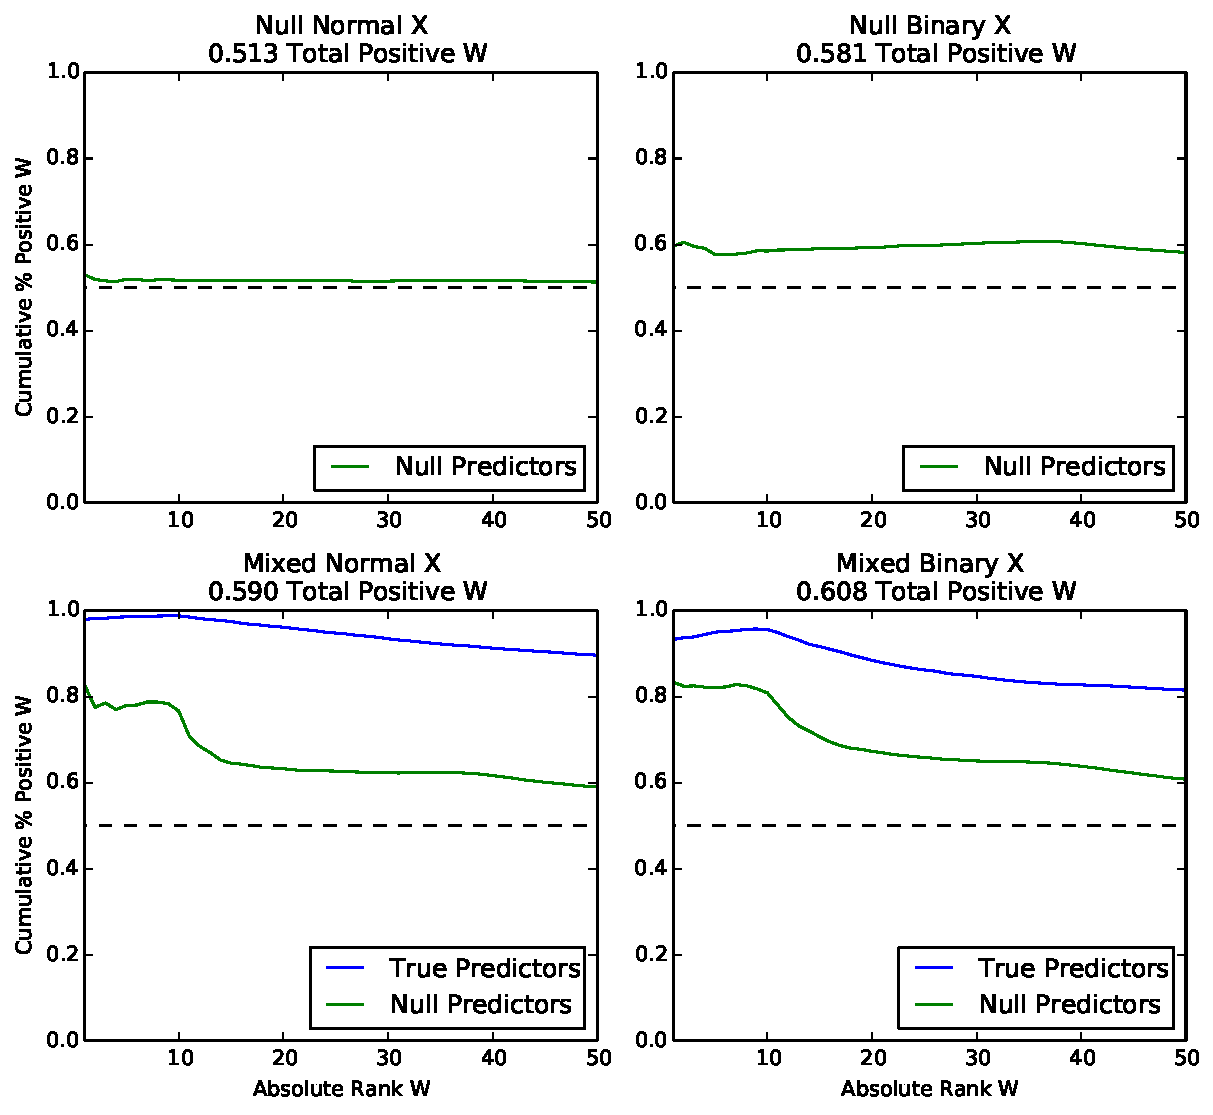
\includegraphics[width=14cm]{images/entryrate_original_logit}
    \end{center}
        \caption{The mean cumulative portion of $W$ statistic which are positive by absolute rank of the value. The mean is over 1000 simulations. On the left side, the features are drawn from a random standard normal distribution. On the right side, they are drawn as Bernoulli with probability $.25$ of being 1. The top has 50 features uncorrelated with the outcome, while the bottom has 40 features uncorrelated with the outcome and 10 correlated with it.}
    \end{figure}
 
    To test how bad this problem is, I tested the method using original style knockoffs in logistic regression. The results can be seen in figure 1, which shows cumulatively, starting with the largest absolute value, what portion of the $W_j$ are positive. For the method to work, for the null predictors, this should be a consistent $50\%$, indicative of the desired symmetric distribution. This is particularly important for high values, which play the largest roll in selecting a threshold. We see that in the top left corner, when all features are null and normally distributed, that we almost achieve this, with only a small, but consistent, deviation from $50\%$. However, in the top right, when the predictors are binary, the null originals enter first far more often, which will result in the FDR being too high. \par
    \FloatBarrier
    This gets much worse when some true predictors are included, as shown in the bottom row of the figure. For both normal and binary predictors, the originals come in first far more often in the beginning. This will completely ruin FDR control, since the portion of null predictors will be assumed far lower than it actually is. It is worth noting that the particular shape of the curve in the diagram, with the plateau for the null predictors through 10, is partially an artifact of how the totals were tabulated. The mean through the first ten is the mean for null predictors that came in first out of both null and true predictors; since the largest ten $W_j$ will tend to be true predictors, the average over the null predictors represent the few extreme $W_j$ which managed to beat out some number of true predictors.  \par
    \begin{figure}[h]
        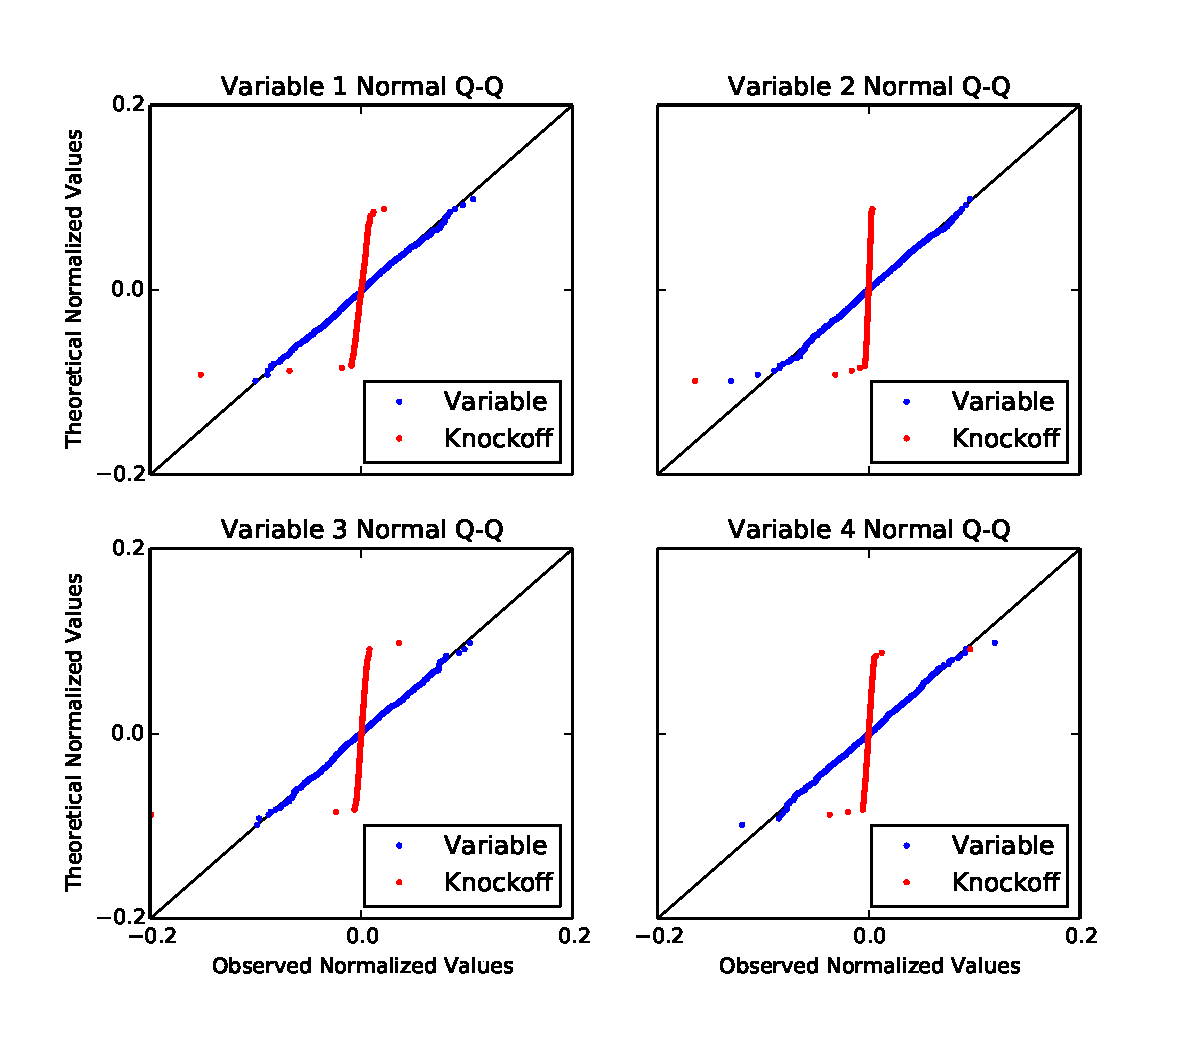
\includegraphics[width=14cm]{images/normalQQ}
        \caption{Normal Q-Q of original variables and knockoffs for simulation with $4$ variables and 1,000 observations}
    \end{figure}


    Upon examination, the issue seems to be that the original style knockoff features have a very different empirical distribution than the features they are imitating. This is obviously true with the binary features, but even with the normal features, the distributions differ a lot. In figure 2, the distribution of four feature and the original style knockoff are plotted against a normal distribution in Q-Q plots. As you can see, they don't match at all. This is suggestive of a solution; if the knockoff variables match the marginal distribution of the original features better, the result may be more suitable for FDR control in GLMs. \par
    \FloatBarrier

\section{Random Binary Knockoffs}
Random binary knockoffs $\mathbf{\tilde x}$, which maintain the correlation condition in expectation, fit the bill in this regard. The method to produce them is based heavily on more general methodology to random binary vector variables with internal correlation.

\subsection{Random Binary Vector Generation}
The full class of random binary vector variables on $\{0,1\}^p$ can be specified as multinomial on the $2^p$ elements of the set. However, in practice, it is generally impractical to specify or estimate all $2^p$ necessary parameters, so it is useful to, as is desirable for knockoffs, pick a method to match the first two moments. These are the mean vector $\E(\bf x)=m\in(0,1)^p$ and the cross-moment matrix $\E(\bf x\bf x^T)=M\in(0,1)^{p\times p}$. Obviously, $m_i = \p(x_i=1)$, $M_{ij} = \p(x_i=x_j=1)$, and $\mathbf m=\diag{M}$. For an arbitrary symmetric $M$ to be valid cross-moment matrix for some random binary vector variable, $M-mm^T\succeq0$, and
    \[ \max\{0,m_i+m_j -1\} \leq M_{ij} \leq \min\{m_i,m_j\}\]
    for all $i\neq j.$ Given a qualifying $M$, or observed $X$, there are then a few methods for generating additional random values.

\subsubsection{Gaussian Copula Family}
Since multivariate normal distributions are easy to randomly draw from and defined by their first two moments, an obvious choice is to use them to generate random binary vectors. This might be done by finding $\mu$ and $\Sigma$ such that for $\mathbf z\sim N_p(\mu,\Sigma)$, $x_i$ can be generated as $x_i = \mathrm{sign}(z_i)$, and have the desired first two moments. However, this is only guaranteed to be feasible in the bivariate case. For higher dimensions, this method can generally only provide random binary vectors with approximately the right moments, and the quality of the approximation quickly degenerates as $p$ increases.

\subsubsection{$\mu$-Conditionals family}
    There exists a more flexible family which will always work for arbitrary $M$ called $\mu$-conditionals. The basic idea is that the $X$ is generate sequentially as 
    \[ \p(x_{i}=1\st x_{1},...,x_{i-1}) = \mu\left(a_{ii}+\sum_{k=1}^{i-1}a_{ik}x_i\right) \]
    for some monotone function $\mu:\R\to(0,1)$. This is essentially a binomial family GLM for a link function $\mu$. If one takes all of the $a_{kj}$, they can form a lower triangular matrix $A$, and then the joint density can be expressed as 

    \[ \p(\mathbf x=\mathbf \gamma) \propto \mu(\mathbf{\gamma}^T A\mathbf \gamma)\]

    If $\mu$ is chosen such that it is a bijection and differentiable, there is a unique $A$ such that $\E(\mathbf x \mathbf x^T)=M$ when generated from this model. The natural choice for $\mu$ is the logistic link function $L(x)=\frac{1}{1-e^{-x}}$, which yields the Ising model, the ``binary analogue of the multivariate normal distribution which is the maximum entropy distribution on $\R^p$ having a given covariance matrix." Additionally, it has the usual benefit that the coefficients can be viewed as a log odds ratio:
    \[a_{ij} = \log\left(\frac{\p(x_j=x_k=1)\p(x_j=x_k=0)}{\p(x_j=0,x_k=1)\p(x_j=1,x_k=0)}\right) \]
    when $i\neq j$. When $\bf x$ is generated from this model with $a_{ij}=0$, then $x_i$ and $x_j$ are conditionally independent.  \par

    There is no closed form to calculate the entries in $A$ if $p>1$, but they can be derived numerically two ways. The first of these, when one is attempting to replicate the empirical cross-moments from a data matrix $X$, $a_{1i}$ to $a_{ii}$ is by fitting successive binomial family GLM regressions. The link function is the given function $\mu$, and $X_i$ is regressed on $X_{1} \ldots X_{i-1}$ using maximum likelihood. $a_{ji}$ for $i\neq j$ will then be the coefficient on $X_j$ while $a_{ii}$ is the intercept of the regression. \par
    Otherwise, if one is just working with a desired cross-moment matrix $M$, the successive rows of $A$ can be fit via Newton-Raphson. This is performed successively on each row of $A$. If the first $i-1$ rows have been fit, then the upper left $(i-1)\times(i-1)$ sub matrix $A_{-i}$ of $A$ has already been filled. Next, $\mathbf a_i$, the first $i$ entries of the $i$th row of $A$ must be fit, while the rest of the row will be 0. This corresponds to $\mathbf m_i$, the first $i$ entries of the $i$th row of $M$. In other words, $\mathbf{m}_i = [\E(x_i x_j)]_{j=1}^{i}$. Finally, let us say that $\mathbf x_{-i}$ is the first $i-1$ entries of $\mathbf x$. $\mathbf a_i$ must satisfy 
            \begin{align*}
                \mathbf m_i &= \E\left(x_i \left[\begin{array}{c} \mathbf x_{-i} \\ x_i \end{array}\right]\right) \\
                \mathbf m_i &= \E\left(\E\left(x_i \left[\begin{array}{c} \mathbf x_{-i} \\ x_i \end{array}\right]\;\bigg \vert\; \mathbf x_{-i}\right)\right)\\
                \mathbf m_i &= \sum_{\mathbf x_{-i} \in \{0,1\}^{i-1}} \p(\mathbf x_{-i})\p(x_i=1\st \mathbf x_{-i}) \left[\begin{array}{c} \mathbf x_{-i} \\ 1 \end{array}\right] \\
            \end{align*}
            When $\mu$ is the logistic link function $L$, this is
            \[ \mathbf m_i = \sum_{\mathbf x_{-i} \in \{0,1\}^{i-1}} \frac{1}{c}L\left(\mathbf x_{-i}^TA_{-i}\mathbf x_{-i}\right) L\left(\mathbf{a}_i^T\left[\begin{array}{c} \mathbf x_{-i} \\ 1 \end{array}\right]\right)\left[\begin{array}{c} \mathbf x_{-i} \\ 1 \end{array}\right] \]
            Where $c$ is the appropriate normalizing constant. Let us define the quantity on the right in the last line as $f(\mathbf a_i)$. This equation $f(\mathbf a_i)=\mathbf{m}_i$ can be solved by successive Newton-Raphson iterations defined by 
            \[\mathbf a_i^{(k+1)} = \mathbf a_i^{(k)} - \left[J\left(\mathbf a_i^{(k)}\right) \right]^{-1}\left[f\left(\mathbf a_i^{(k)}\right)-\mathbf m_i\right] \]
            where $J$ is the Jacobian of $f$. To do so, the Jacobian matrix is calculated as 
        \[ J\left( \mathbf a_i\right) = \sum_{\mathbf x_{-i} \in \{0,1\}^{i-1}} \frac{1}{c}L \left(\mathbf x_{-i}^TA_{-i}\mathbf x_{-i}\right) L'\left(\mathbf{a}_i^T\left[\begin{array}{c} \mathbf x_{-i} \\ 1 \end{array}\right]\right)\left[\begin{array}{c} \mathbf x_{-i} \\ 1 \end{array}\right]\left[\begin{array}{cc} \mathbf x_{-i}^T & 1 \end{array}\right] \]
            With $2^{i-1}$ possible values for $\mathbf x_{-i}$, this can quickly become computationally expensive. Instead, with a series of values $\mathbf x_{-i}^{(k)}\sim \mathbf x_{-i}$, the simulated values 
            \[f\left(\mathbf a_i\right) \approx \frac{1}{K}\sum_{k=1}^K L\left(\mathbf{a}_i^T\left[\begin{array}{c} \mathbf x_{-i}^{(k)} \\ 1 \end{array}\right]\right)\left[\begin{array}{c} \mathbf x_{-i}^{(k)} \\ 1 \end{array}\right] \]
            and
            \[J\left( \mathbf a_i\right) \approx \frac{1}{K}\sum_{k=1}^K L'\left(\mathbf{a}_i^T\left[\begin{array}{c} \mathbf x_{-i}^{(k)} \\ 1 \end{array}\right]\right)\left[\begin{array}{c} \mathbf x_{-i}^{(k)} \\ 1 \end{array}\right]\left[\begin{array}{cc} \mathbf [x_{-i}^{(k)}]^T & 1 \end{array}\right] \]
            can be used. \par
            Though, in theory, $A$ should always exist, in practice limited accuracy may dictate that Newton-Raphson method won't converge. In the simulation method in particular, if $K$ is not large enough, the equations can be very difficult or impossible to solve. When the intial problem can't be solved, besides increasing the simulation size or numerical accuracy, one can instead solve the relaxed problem  $f(\mathbf a)=\mathbf m_i^*(\tau)$, where, for $\tau\in[0,1]$
    \[\mathbf m_i^*(\tau) = (1-\tau)\mathbf m_i + \tau \left[ \begin{array}{cccc} 0 & \ldots & 0 & M_{ii} \end{array} \right]^T \]
            When $\tau=0$, this yields the original problem, while when $\tau=1$, it is treats $x_i$ as independent of $\mathbf x_{-i}$. The latter will always have the solution
            \[\mathbf a_i = \left[ \begin{array}{cccc} 0 & \ldots & 0 & \log\left(\frac{M_{ii}}{1-M_{ii}}\right) \end{array} \right]^T \]
            The hope is that for some $\tau$ close to $0$, convergence can be achieved, only causing a slight distortion from the desired cross moments.

\subsection{Generating Binary Knockoffs}
This theory provides the tools to generate random binary knockoffs. This is done is done sequentially as two steps, the first of which is to come up with the target covariance matrix $\Sigma_L$ for $\mathbf x_L = [\mathbf x\; \mathbf{\tilde x}]$. This is extremely similar, though not identical, to the method with the original knockoffs, where $X_L^TX_L$ after normalization was targeted. However, much the same method as before can be used. Let the vector of empirical means of the columns of $X$ is $\mathbf m = \frac{1}{n}X^T\mathbf 1$ and the empirical covariance matrix of $X$ is $\Sigma = \frac{1}{n}X^TX - \mathbf{m}\mathbf{m}^T$. Much as before with the original knockoffs, both the equi-correlated and SDP method can be used to select  $\mathbf s$  such that $\diag{\Sigma}-\mathbf s$ is small and 
        \[ \Sigma_L = \left[\begin{array}{cc}  \Sigma & \Sigma - \diag{\mathbf s }\\ \Sigma - \diag{\mathbf s} & \Sigma \end{array}\right] \succeq 0 \]
    While with the original knockoffs, the result was small values for $X_i^T\tilde X_i$, now the result is low covariance between $x_i$ and $\tilde x_i$.\par
    Additionally though, the moment condition must hold for $\Sigma_L$ to correspond to a proper random binary vector. If $\mathbf m_L = \E\left(\mathbf x_L\right) = [\mathbf m \; \mathbf m]$, then the desired cross moment matrix of the joint distribution is 
        \[ M_L = \Sigma_L + \mathbf m_L\mathbf m_L^T\]
        So it must be the case that  
        \[\max\{0,\mathbf m_{L,i} + \mathbf m_{L,j} -1\} \leq \Sigma_{L,ij} + \mathbf m_i \mathbf m_j \leq \min\{\mathbf m_{L,i}, \mathbf m_{L,j}\} \]
        However, since $\Sigma$ and $\mathbf m$ are from an actual random binary vector, the entries of $\Sigma$ satisfy this property by default. Only off diagonal entries which have had $\mathbf s$ subtracted from them could possibly violate this condition. Furthermore, for these entries, the goal is to make $\Sigma_{L,ij}$ as close to $0$ as possible. Since the condition is always satisfied in a neighborhood of $M_{L,ij} = \mathbf m_{L,j}\mathbf m_{L,i}$, this implies that this method should normally be satisfied. This is the principle advantage minimizing the $\textrm{cor}(x_i,\tilde x_i)$ rather than $\E[x_i\tilde x_i]$. For the SDP method though, the restriction can be built directly into the optimization problem. If $\sigma = \diag{\Sigma}^{\frac{1}{2}}$ is the vector of standard deviations, the updated problem is
            \begin{center}
                \begin{tabular}{r l}
                    minimize & $\|\mathbf 1-\diag{\sigma}^{-1}\mathbf s\|_1$ \\
                    subject to & $ 0 \preceq \diag{\mathbf s} \preceq 2\Sigma $ \\
                               & $ 2\mathbf m_i -1 \leq \Sigma_{ii}-\mathbf s_i + \mathbf m_i^2 \leq \mathbf m_i  \quad \forall i$
                \end{tabular} 
            \end{center} 
            the factor of $\diag{\sigma}^{-1}$ in the objective is to account for the $x_i$ not being normalized, as was the case with the original knockoffs. \par
\subsubsection{Fitting via $\mu$-conditionals}
        Once a proper cross moment matrix $M_L$ has been selected, the most obvious approach to generate knockoffs is to apply the Newton-Raphson method to fit the matching $A$ matrix. This can be used to generate $\mathbf{ \tilde x}$ sequentially conditioned on $x$, as $\tilde x_i \st \mathbf x,\tilde x_1,\ldots,\tilde x_{i-1}$. However, there are a few variations of this process which are preferable depending on the situation. 
        \begin{enumerate}
            \item If the whole $A$ matrix is being fit, then the upper half of the matrix, corresponding to $\mathbf x$, can be fit via the regression method, since they arise from real data $X$. This will tend to be quicker, since the calculation lends itself to parallel computing, and the data set will often be smaller than the space of all binary vectors or a simulation of that space. The second half of the matrix still must be fit via Newton-Raphson.
            \item One can avoid fitting the first half of the $A$ matrix entirely though if performing Newton-Raphoson with by using the actual observed values in $X$ to simulate the first half of $\mathbf x_L$. This can be done by either bootstrapping rows from $X$ or using some number of copies of $X$ exactly. The advantage of this is the saved computation and that $\tilde x$ should be built to match the correlation condition more exactly. The downside is that, since these values won't be from the Ising model, the theoretical guarantee of a suitable $A$ may no longer hold. As well, if $n$ isn't big enough, the equations will quickly become difficult to solve, since the observed samples will provide a noisy and incomplete sample of the probability space.
            \item As $A$ is being fit, even the parts of $\mathbf x_{-i}$ corresponding to knockoffs need not be redrawn for each Newton-Raphson iteration or each successive $i$. To fit $\mathbf a$ for feature $i$, the $\mathbf x_{-i}^{(k)}$ will remain constant; then, once $\mathbf a$ has been fit, the $x_i^{(k)}$ need only be drawn once. This saves computation, and the multiplication
            \[ \left[\begin{array}{c} \mathbf x_{-i}^{(k)} \\ 1 \end{array}\right]\left[\begin{array}{cc} \mathbf [\mathbf x_{-i}^{(k)}]^T & 1 \end{array}\right] \]
                needs only be partially recalculated for each Newton-Raphson iteration since the upper left portion, $\mathbf x_{-i}^{(k)}[\mathbf{x}_{-i}^{(k)}]^T$, won't change. This may result in slight deviations in any particular draw compounding into a more severe error over time.
            \item As $p$ grows large, and $K$ necessarily along with it, the cost of calculating the Jacobian matrix grows far quicker than the cost of calculating $f(\mathbf a)$. This is since it has $O(Kp^2)$ complexity compared to $O(Kp)$ complexity for $f(\mathbf a)$. This can quickly become prohibitive. One might instead estimate the full Jacobian based on first differences, but in practice Anderson Mixing, a quasi-Newtonian method, works well. In general, quasi-Newtonian methods perform Newton-Raphson iterations but replace the full inverted Jacobian at each itteration $k$ with an approximation $G_k$. Thus, to solve for a variable $\mathbf z$ such that $f(\mathbf z)=\mathbf 0$, the best approximation for the zero is updated as $\mathbf z_{k+1}=\mathbf z_k - G_k f(\mathbf{z}_k)$. \par
    Anderson mixing does this implicitly, with no extra recalculation of $f$, by approximating $f$ with the affine space spanning the previous $m$ evaluations of $f$, at $\mathbf z_{k}$ through $\mathbf z_{k-m+1}$. The best approximation for $f(\mathbf z)=0$ in this space is defined by
    \[ \mathbf \alpha = \argmin_{\|\mathbf w\|_1=1} \|\sum_{i=1}^m f(\mathbf z_{k-i+1}) w_i \|_2 \]
    This leads to the updated approximation
    \[ \mathbf z_{k+1} = \sum_{i=1}^{m} w_i \mathbf z_{k-i+1} \]
    There is no explicit calculation of $G_k$ needed here, and to do so in practice would be slower. However, it's presence can be seen through an equivalent formulation. Let 
    \[ \mathcal F = [(f(\mathbf z_k) - f(\mathbf z_{k-1})) \ldots (f(\mathbf z_k) - f(\mathbf z_{k-m}))] \]
    and
    \[ \mathcal Z = [(\mathbf z_k - \mathbf z_{k-1})\ldots (\mathbf z_k - \mathbf z_{k-m})] \]
    This means $\mathbf \alpha$ is now
    \[ \mathbf \alpha \; = \;\argmin_{\|\mathbf w\|_1=1} \|f(\mathbf z_{k}) - \mathcal  F \mathbf w\|_2\; = \;(\mathcal F^T \mathcal F)^{-1}\mathcal F^T\mathbf z_k \]
    so 
    \[ \mathbf z_{k+1} \;= \;\mathbf z_{k+1} - \mathcal Z \alpha\; = \;z_{k+1} + \mathcal Z(\mathcal F^T \mathcal F)^{-1}\mathcal F^T\mathbf z_k \]
    Which yields the approximated inverse Jacobian $G_k= \mathcal Z(\mathcal F^T \mathcal F)^{-1}\mathcal F^T$
        \end{enumerate}
        In practice, it seemed that combining the first, third, and fourth variation was the most successful technique. However, should $n$ be sufficiently large, the second variation also saves a lot of time. 

\subsubsection{Fitting via Quadratic Programing}

        Random binary knockoffs which produce the desired cross moment matrix $M_L$ need not arise from a generative model for $\mathbf{\tilde x}$ however. It is sufficient to have a random matrix $\tilde X \in \{0,1\}^{n\times p}$ such that 
        \[ \E_{\tilde X}(X^T \tilde X) = \Sigma - \diag{s} \quad \& \quad \E_{\tilde X}(\tilde X^T \tilde X) = \Sigma\]
        The simplest way to do this is based on a probability matrix $P\in (0,1)^{n\times p}$ where each $X_{ij}$ is drawn independently as $X_{ij}\sim\textrm{Bernoulli}(P_{ij})$. This requirement can be stated as the quadratic feasibility problem
            \begin{center}
                \begin{tabular}{r l}
                    exists     & $P$ \\
                    subject to & $X^TP=\Sigma-\diag{s} $ \\
                               & $P^TP=\Sigma $ \\
                               & $0 \leq P \leq 1$
                \end{tabular} 
            \end{center}
        If such a matrix exists and can be found, then $\tilde X$ can easily be generated. However, the constraints likely result in infeasibility much of the time. Instead, one can try to minimize how far the expected moments given $P$ would be from those desired for $M_L$. Ideally, this would take the form
            \begin{center}
                \begin{tabular}{r l}
                    minimize     & $\|X^TP-(\Sigma-\diag{s})\|_{fro}^2 + \|P^TP-\Sigma\|_{fro}^2 $\\
                    subject to   & $ \mathbf 1^T P = \mathbf m_L $ \\
                                 & $0 \leq P \leq 1$
                \end{tabular} 
            \end{center}
            Here, the marginal distribution of $\tilde X_i$ will be the same as $X_i$, and the crossmoments shouldn't deviate to far from $M_L$. This problem can be stated as the quadratic program via the introduction of slack variables:
            \begin{center}
                \begin{tabular}{r l}
                    minimize     & $\|W\|_{fro}^2 + \|V\|_{fro}^2 $ \\
                    subject to   & $ -W \leq X^TP-(\Sigma-\diag{s})\leq W $ \\
                                 & $ -V \leq P^TP-\Sigma \leq V $ \\
                                 & $ \mathbf 1^T P = \mathbf m_L $ \\
                                 & $0 \leq P \leq 1$
                \end{tabular} 
            \end{center}
            Though there are nice tools and theory for solving quadratic programs, $n\times p$ would have to be fairly small for this optimization problem to be computationally reasonable in practice. Ideally, there would be a method to breakdown this problem into a series of smaller optimization problems which would yield the same solution. An optimist might hope that iterating through the columns of $P$, optimizing each to hit its desired crossmoments individually conditioned on the estimate of the rest of $P$, would achieve this. In practice, this does seem to yield reasonable results, and is far quicker than other methods for large $p$.In particular, this method seemed to work well:
    \begin{enumerate}
        \item Optimize initial $P_i$ as such that $X_j^T P_i = M_ij$ if $i\neq j$ and $X_i^T P_i = \sigma_i(1-s)$.   
            \begin{center}
                \begin{tabular}{r l}
                    minimize     & $ \left(\frac{1}{n}X_i^T P_i - (M_{ij}-\sigma_i(1-s))\right)^2 + \sum_{i\neq j}(\frac{1}{n}X_j^T P_i - M_ij)^2$ \\
                    subject to   & $ \frac{1}{n}\mathbf 1^T P_i = M_{ii} $ \\
                                 & $0 \leq P_i \leq 1$
                \end{tabular} 
            \end{center}
        \item Draw initial $\tilde X_i$ as independent Bernoulli with probability $P_i$.
        \item Iterate through $1\leq i \leq p$, fitting new $P_i$ such that 
            \begin{center}
                \begin{tabular}{r l}
                    minimize     & $ \left(\frac{1}{n}X_i^T P_i - (M_{ij}-\sigma_i(1-s))\right)^2 + \sum_{i\neq j}(\frac{1}{n}X_j^T P_i - M_ij)^2 + \sum_{i\neq j}(\frac{1}{n}\tilde X_j^T P_i - M_ij)^2$  \\
                    subject to   & $ \frac{1}{n}\mathbf 1^T P_i = M_{ii} $ \\
                                 & $0 \leq P_i \leq 1$
                \end{tabular} 
            \end{center}
    \end{enumerate}

            




\section{Binary Knockoff Performance}
    To evaluate how useful these binary knockoffs will be in practice, it is useful to evaluate their empirical performance under simulation. 

\subsection{Convergence to Theoretical Covariance} 


\end{document}
